%\documentclass{recpad2k}
\documentclass[extendedabs]{recpad2k}
\usepackage[T1]{fontenc} 
\usepackage[utf8]{inputenc}
\usepackage{amsthm}
\usepackage{amsfonts}
\usepackage{enumitem}
\usepackage[font=small,labelfont=bf]{caption}
\usepackage{floatrow}
\usepackage{etoolbox}
\usepackage{blindtext}
\usepackage[compact]{titlesec}
    \titlespacing*{\section}{-10pt}{-10pt}{-\parskip}
    \titlespacing*{\subsection}{-10pt}{-10pt}{-\parskip}
         \setlength{\parskip}{0cm}
    \setlength{\parindent}{1em}
\setlist[itemize]{noitemsep, topsep=0pt}

\makeatletter
\g@addto@macro\normalsize{%
    \setlength\belowdisplayskip{-0pt} \setlength\abovedisplayskip{-0pt}
}
\patchcmd{\@maketitle}
  {\addvspace{0.5\baselineskip}\egroup}
  {\addvspace{-1\baselineskip}\egroup}
  {}
  {}
\makeatother
%% Enter your paper number here for the review copy
\recpadreviewcopy{??}

\title{Selection of the number of states in hidden semi-Markov models}


% Enter the paper's authors in order
% \addauthor{Name}{email/homepage}{INSTITUTION_CODE}
\addauthor{Filipa Rente}{filipaoliveirarente@gmail.com}{1}
\addauthor{Zita Marinho }{zam@priberam.pt}{2}
\addauthor{Mário Figueiredo}{ mario.figueiredo@tecnico.ulisboa.pt}{3}

% Enter the institutions
% \addinstitution{Name\\Address}
\addinstitution{
 Instituto Superior Técnico (IST),\\ 
 Universidade de Lisboa (ULisboa), Portugal
}
\addinstitution{
Instituto de Sistemas e Robótica, IST \\
Priberam Labs, Lisboa, Portugal
}
\addinstitution{
 Instituto de Telecomunicações, \\
 IST, ULisboa, Portugal
}

\runninghead{Student, Prof, Collaborator}{RECPAD Author Guidelines}

% Any macro definitions you would like to include
% These are not defined in the style file, because they don't begin
% with \bmva, so they might conflict with the user's own macros.
% The \bmvaOneDot macro adds a full stop unless there is one in the
% text already.
\def\eg{\emph{e.g}\bmvaOneDot}
\def\Eg{\emph{E.g}\bmvaOneDot}
\def\etal{\emph{et al}\bmvaOneDot}

%------------------------------------------------------------------------- 
% Document starts here
\begin{document}

\maketitle

\begin{abstract}
%The order selection problem is of crucial importance for many statistical models.
This paper addresses the order selection problem for Hidden semi-Markov models (HSMMs). We propose a novel approach to select the optimal number of states, as well as the state duration of an HSMM. One of the main contributions of this paper is a proof of an equivalence of models which allows us to focus only on the selection of the number of states. We propose a unique order selection criterion based on that proof. %The literature is divided into two different approaches. The first uses model selection methods to select a fixed number of states, while the second is based on the Bayesian setting where these hyper-parameters are treated as unknown random variables and are estimated during the training process. This paper proposes
Furthermore, the optimal number of states is found through a sequential pruning strategy using a mixture minimum description length (MMDL) criterion, based on \citet{figueiredo1999fitting}, for mixture models, and \citet{bicego2003sequential} for Hidden Markov models (HMMs). We demonstrate the effectiveness of the approach using synthetic experiments. Source code available at \url{https://github.com/filiparente/hsmm_mmdl}.\\ \noindent
\textit{Keywords}: Hidden semi-Markov models; Order selection problem; Minimum description length; Bayesian inference criterion; State pruning.
\end{abstract}
\vspace*{-3pt}
\section{Introduction}
\label{sec:intro}
HSMMs are an extension of Hidden Markov Models (HMMs) where the state duration is explicitly modelled. State duration distributions can be non-parametric (multinomial) or parametric. The duration in a $k$-state HMM is implicitly a geometric distribution with parameter $A_{ii}, \forall{i\in [k]}$, which corresponds to the diagonal entries of the transition probability matrix $\boldsymbol{A}\in \mathbb{R}^{k\times k}$. %Therefore, the probability of duration $d$ in state $s_i, \forall{i\in[k]}$  ($p_i(d)$) is given by the geometric probability of $d-1$ times in the same state which correspond to $d-1$ failures before the first success, where the success is in fact a transition to another state. That is, $ p_i(d)=(1-A_{ii}^{d-1})A_{ii}$.
This implicit modeling of state duration is not sufficient for many real problems. Consequently, for those problems a model such as HSMMs is more suitable to provide a higher expressiveness to the state duration modeling. One example include time series segmentation of human motion data into single actions, where the probability distribution used for the duration is extremely important in order to correctly cluster the different motion activities \cite{nakamura2017segmenting}. %Another interesting example of the use of HSMM to model the duration explicitly is in \citet{chen2015estimating}, where the author adopt non-parametric durations to estimate the latent sequence of attentional states in a identification task with mice. 
%The observations are the (continuous) reaction time of the mice to visual stimulus and a binary variable of whether they made the correct or the wrong decision based on the visual stimulus. The estimated sequence of the latent attentional states model the neurological behavior of the mice, again being the state duration modeling an important aspect for the achievement of high estimation accuracy. 
\vspace*{-2pt}
\section{Hidden semi-Markov models}
\label{sec:hsmm}
A hidden semi-Markov model is a probabilistic model in which a stochastic sequence of observations $\textbf{O}=O_{1:T}$ is generated by an hidden random sequence $\textbf{S} = S_{1:T}$, where $O_t$ denotes the observed symbol at time $t$ and $S_t$ the state occupied by the system at time $t$. A $k$-state HSMM is completely defined by $\mu=(\mathbf{s}, A, \boldsymbol{\pi}, B, D)$:
%\begin{itemize}

    \textbullet  A set $\mathbf{s}=\{s_1,...,s_k\}$ of hidden states and a set $\{o_1,...,o_m\}$ of observation symbols;
    
    \textbullet  A transition matrix ${A}\in \mathbb{R}^{k^2 \times {d_{max}}^2}$, whose element $A_{id',jd}$ represents a transition from state $s_i$ with duration $d'$ to state $s_j$ with duration $d$,
    \begin{equation}
        A_{id',jd} = \mathbb{P}[S_{t+1}=s_j, \tau_{t+1}=d|S_t=s_i, \tau_t=d'],
        \label{A-hsmm}
    \end{equation}
    where $\tau_t$ represents the residual time in state $S_t$ and  $i,j \in [k]$ and $d,d' \in  [d_{max}]$. Here, the explicit duration HMM variant of HSMMs will be considered, which assumes that a state transition is not dependent on the duration of the previous state. Thus, eq. \eqref{A-hsmm} simplifies to
    \begin{equation}
        A_{id',jd} = A_{i,jd} = A_{ij}p_j(d),
    \end{equation}
    where $A_{ij}$ is the transition probability matrix as in HMMs and $p_j(d)$ is the explicit state duration probability;
    
    \textbullet  An emission matrix $B\in\mathbb{R}^{k\times m}$ which represents
    \begin{equation}
        B_{ij}=\mathbb{P}[O_t=o_j|S_t=s_i]
    \end{equation}
    the probability of observing symbol $o_j$ while in state $s_i$.  Here, we opted for a parametric Poisson emission distribution. That is,
    \begin{equation}
        \mathbb{P}[o_j|s_i] = \dfrac{\lambda_i^{o_j} e^{-\lambda_i}}{o_j!},
        \label{poisson}
    \end{equation}
    where $\lambda_i$ is the Poisson parameter associated with state $s_i$;
    
    \textbullet  An initial state probability $\boldsymbol{\pi}\in\mathbb{R}^{k}$ with elements $\pi_i=\mathbb{P}[S_1=s_i]$;
    
    \textbullet A duration probability matrix $\boldsymbol{D}\in \mathbb{R}^{k\times d_{max}}$ where $D_{jd}=p_j(d)$ is the probability of occupying state $s_j$ with duration $d$. Here, we also considered a parametric distribution as a mixture of geometric distributions,
    \begin{equation}
        p_j(d) = \sum_{m=1}^{M_j} c_{jm} \text{Geom}(d|\theta_{jm}),
        \label{mix_geom}
    \end{equation}
    where $\text{Geom}(d|\theta_{jm})$ denotes a geometric density with parameter $\theta_{jm}$ for state $s_j$ and component $m$. The durations in state $s_j$ are modelled as samples from a geometric mixture with $M_j$ components, with $c_{jm}$ being the mixing weight of the $m^{th}$ component in state $s_j$. One of the main contributions of this paper is a proof that an HSMM where the state duration distribution is a mixture of geometric distributions (for each state) is equivalent to another HSMM with only one geometric distribution $p_{jm}(d)$ per state $s_{jm}$, but more states. That is, the set of states $\mathbf{s}$ is augmented to $\mathbf{s'}$ in this equivalent model.\footnote{$\mathbf{s'}=\{s'_1,...,s'_{k'}\}=\{s_{11},...,s_{1M_1},...,s_{jm},...,s_{k1},...,s_{kM_k}\}$, where $k'=\sum_{j=1}^k M_j$ is the (augmented) number of states of the equivalent model.} %A formal proof of this equivalence can be found in Appendix A.
    Using this result, we will consider only HSMMs with one geometric duration distribution for each state. That is, %with geometric probability mass function
    \begin{equation}
        p_{jm}(d) = \text{Geom}(d|\theta_{jm}) = (1-\theta_{jm})^{d-1}\theta_{jm}, \qquad 1\leq d \leq d_{max}.
    \label{geom}
    \end{equation}
    
    \textbullet Hyperparameters: the number of states $k$, and the maximum allowed duration $d_{max}$. $d_{max}$ is used to truncate the forward-backward pass in the EM algorithm, and it represents the maximum number of observations within all states. The number of states is estimated using the sequential pruning strategy with the MMDL criterion, described in Section \ref{sec:order}.
%\end{itemize}

\section{Order estimation for HSMMs}
\label{sec:order}
The order estimation problem in HSMMs consists of estimating the optimal number of states ($k^*$) and maximum allowed state duration (${d_{max}}^*)$.  Hence, the order estimation procedure is a multivariate optimization problem where we optimize both $k$ and $d_{max}$ w.r.t. the same criterion. 
One greedy approach would be to try every possible combination of $k$ and $d_{max}$ and assign the one with the highest model likelihood. %Another possible solution is to optimize $k$ and $d_{max}$ separately, but concerning the same criterion. However, the solution we would get would not be the optimal one because for optimizing one parameter we would need to fix the other in a (probably) non-optimal value. 
Ideally, it would be better to guarantee that each state is connected to the set of possible durations $\{1,2,...,d_{max}\}$ in a one-by-one relationship.  This result would allow the problem to be simplified to a univariate optimization problem, where the focus is only on the selection of $k^*$. If we consider a model with high statistical complexity, e.g., with non-parametric (multinomial) state duration distributions, then this one-by-one relationship is not present, because each state needs $d_{max}$ "parameters" to specify its duration. Likewise, one can consider a model with lower statistical complexity, i.e., with parametric state duration distributions, where, in analogy with the multinomial case, each state has a mixture of parametric distributions for its duration probability (e.g. a mixture of geometric distributions). Nonetheless, the problem remains since each state has multiple parameters (as many as the number of components of the mixture of that state) to specify its duration. Fortunately, the equivalence of models (proof omitted due to space constraints) allows us to consider instead an equivalent model with more states (augmented states) but only one geometric distribution per state. Consequently, each state has one and only one parameter to specify its duration (the parameter of the geometric distribution), therefore guaranteeing the one-by-one relationship required. Using this equivalent model, $d_{max}$ can be empirically estimated through the parameters of the geometric distributions. In fact, there is a correspondence between the parameter $\theta_{jm}$ of the geometric distribution (of state $s_{jm}$) and the durations $d$: a lower parameter is associated with higher durations. Therefore, $d_{max}$ can be estimated through the following steps: (1) find the lowest parameter $\theta_{jm}$ between all states $\mathbf{s'}$; (2) find the duration for which the cumulative probability (easily derived from the PMF of eq. \eqref{geom}), with parameter found in (1), is smaller than $\epsilon$.\footnote{A reasonable value for $\epsilon$ is of the order of $0,01$.} After determining the hyper-parameter $d_{max}$, the state duration probability matrix $\boldsymbol{D} \in \mathbb{R}^{k \times d_{max}}$ (used in the EM algorithm) can be filled with values from the geometric PMF (eq. \eqref{geom}) evaluated at the corresponding durations $d=1,...,d_{max}$. \\ \noindent
In the following sections, we will discuss the adaptation of two different selection criteria to the HSMM setting: Bayesian inference criterion (BIC) and mixture minimum description length (MMDL).
\subsection{Bayesian inference criterion (BIC)}
The BIC criterion for $k$ states is generally defined as
\begin{equation}
    \text{BIC}(k) = \log \mathbb{P}[\textbf{O}|\hat{\mu}_k]-\dfrac{N_k}{2}\log(n),
    \label{bic}
\end{equation}
where the first term is the log-likelihood of the observations ($\textbf{O}$) given the maximum likelihood estimated parameters by the EM algorithm ($\hat{\mu}_k$), hereinafter referred to as $\text{LL}$. The second term penalizes the model complexity through the total number of free parameters $N_k$ weighted by the total number of observations $n$. %If the observations are sequences of $N$ observations of the same length $l$, then $n=N\times l$, otherwise $n=\sum_{h=1}^N l_h$, where $l_h$ is the length of the $h^{th}$ sequence of observations.
The optimal number of states is the one that maximizes the criterion in eq. \eqref{bic}, i.e., $\hat{k}_{\text{BIC}} = \arg \max_k \text{BIC}(k)$. For HSMMs, the BIC criterion is the one in eq. \eqref{bic} with $N_k$ decomposed in terms of the number of free parameters for each variable ${N_k}^{\boldsymbol{A}}+{N_k}^{\boldsymbol{\pi}}+{N_k}^{\boldsymbol{B}}+{N_k}^{\boldsymbol{D}}$. The number of free parameters for the transition matrix is ${N_k}^{\boldsymbol{A}}=k(k-2)$ since: (1) it is a stochastic matrix %, hence $\sum_{j=1}^k A_{ij}=1$, which means that one element in every row is dependent on the others,
and (2) the diagonal entries are zero, $A_{ii}=0$, because in HSMMs no self-transitions are allowed due to the explicit specification of state durations. For the initial state distribution, ${N_k}^{\boldsymbol{\pi}}=k-1$ and, finally, for the emission and state duration densities, since both are parametric distributions, the total number of free parameters for each is $k$, one per state. To sum up, the general BIC criterion defined in eq. \eqref{bic} is extended to
\begin{equation}
    \text{BIC}_{\text{HSMM}}(k) = \text{LL}-\dfrac{k^2+k}{2}\log(n),
    \label{bic_hsmm}
\end{equation}
where we dropped all terms that do not depend on the number of states $k$.
\subsection{Mixture minimum description length (MMDL)}
This criterion, as the name suggests, is inspired by the Gaussian mixture models (GMMs), where the model complexity penalty term does not need to consider the whole data ($log(n)/2$) given that each component of the mixture is not estimated from all observations but only from those that were in fact generated by that component. Hence, the term $log(n)/2$ is replaced by a quantity that measures how much data was generated by a given component. %, therefore minimizing the length of the amount of description needed for each parameter. 
For GMMs, this quantity is easily obtained as $log(nc_j)/2$, with $c_j$ being the probability of the $j^{th}$ component of the mixture.
For HSMMs, finding this quantity is not so trivial. However, both the transition matrix and the initial state distribution are estimated from the whole data, so those are still weighted by the standard $log(n)/2$ term. On the contrary, the emission probability parameters ($\boldsymbol{\lambda}$) and the state duration probability parameters ($\boldsymbol{\theta}$) are estimated using only the samples from the corresponding component. The quantity that specifies the state probabilities is given by the stationary distribution $\boldsymbol{p}_\infty=[p_\infty(1),...,p_\infty(k)]$\footnote{For HMMs this quantity is obtained from the left eigenvector of the transition matrix A associated with eigenvalue 1.}, which represents the "average" occupation of each (steady) state after the semi-Markov chain has reached its equilibrium. Therefore, for an HSMM with $k$ states, the MMDL criterion is given by
\begin{equation}
    \text{MMDL}_{\text{HSMM}}(k) = \text{LL}-\dfrac{{N_k}^{\boldsymbol{A}}+{N_k}^{\boldsymbol{\pi}}}{2}\log(n)-\dfrac{{N_1}^{\boldsymbol{B}}+{N_1}^{\boldsymbol{D}}}{2}\sum_{m=1}^k log(np_\infty(m)),
    \label{mmdl}
\end{equation}
where ${N_1}^{\boldsymbol{B}}$  and ${N_1}^{\boldsymbol{D}}$ are the number of free parameters of the emission and state duration densities, respectively, of an HSMM with only one state. Since we assumed parametric distributions, ${N_1}^{\boldsymbol{B}}= {N_1}^{\boldsymbol{D}}=1$. Replacing the free parameters in eq. \eqref{mmdl}, yields
\begin{equation}
    \text{MMDL}_{\text{HSMM}}(k) = \text{LL}-\dfrac{k^2-k}{2}\log(n)-\sum_{m=1}^k log(np_\infty(m)).
    \label{mmdl_hsmm}
\end{equation}
\subsection{Stationary probability distribution for HSMMs}
The stationary probability distribution for semi-Markov chains is not the same as for regular Markov chains. However, it can be found empirically. In \cite{barbu2012estimation}, the authors proposed the following estimator
\begin{equation}
    p_\infty(i) = \dfrac{\hat{v_i}(T) \hat{m_i}(T)}{\sum_{i=1}^k  \hat{v_i}(T) \hat{m_i}(T) }, \quad \hat{v_i}(T) = \dfrac{N_i(T)}{N(T)}, \quad \forall i \in [k],
    \label{p_infty_3}
\end{equation}
where $\hat{v_i}(T)$ is an estimator for the stationary probability distribution of the embedded\footnote{The embedded Markov chain of a semi-Markov chain with state sequence $\textbf{Q}=\{4,4,1,1,1,2,3,3,3\}$ is $\textbf{Q'}=\{4,1,2,3\}$ with the corresponding jump times $\textbf{J'}=\{2,5,6\}.$} Markov chain. 
It is obtained from the ratio of the number of visits of the embedded Markov chain to state $s_i$ up to time $T$ ($N_i(T)$) and number of jumps of the embedded Markov chain in the time interval $(0,T]$ ($N(T)$), both available from the estimated state sequence after running the \textit{Viterbi} algorithm. In eq. \eqref{p_infty_3},  $\hat{m_i}(T)$ is an estimator of the mean sojourn time in state $i$, considering all observations up to time $T$. It is obtained by averaging the EM estimate for the state duration probability matrix $\hat{\boldsymbol{D}}$, weighted by the corresponding durations. As desired, the stationary probability distribution for semi-Markov chains $\boldsymbol{p}_\infty$, given by eq. \eqref{p_infty_3}, is a measure of the "average" state occupation.

\subsection{Sequential pruning strategy}
The sequential pruning strategy entails the following steps:
\begin{enumerate}[topsep=0pt,itemsep=-1ex,partopsep=1ex,parsep=1ex]
    \item Set the minimum and maximum allowed number of states: $k_{min}$ and $k_{max}$, respectively;
    \item Initialize the EM algorithm parameters randomly, using $k = k_{max}$ as the initial number of states;
    \item While $k\geq k_{min}$: Run the EM algorithm until convergence and obtain the estimated parameters; Compute and store the value of the model selection criterion given by eq. \eqref{mmdl_hsmm}; Find the least probable state (i.e., the smallest element of $\boldsymbol{p}_\infty$); Prune it by removing the corresponding rows/columns from the estimated parameters; Normalize the estimated parameters that after pruning need normalization\footnote{Set distributions to uniform if normalization is not possible (this problem can arise when considering a large amount of states).}; Set these as the initial parameters of the EM algorithm and set $k=k-1$. Repeat, i.e., run EM again with one less state.
    \item The final model is the one which corresponds to the maximum stored value for the model selection criterion, with the attached optimal number of states $k_*$.
\end{enumerate}
%The reason why this strategy is called "decreasing" learning is because we start with a large number of states and in each iteration we prune the least probable state of the model, resulting in a reduced model which is used as the initial configuration for the next EM training, with one less state. This strategy guarantees a lower sensitivity to the initialization of the EM algorithm given that in each iteration we initialize in a better situation after removing the least probable state.

\section{Results with synthetic data}
The synthetic data corresponds to 2 sequences of 1000 observations each sampled from an HSMM with random parameters $\mu$ and 5 states. According to the results shown in Fig.1, the standard BIC retrieves an expected number of states 4.42 on average over 50 runs, while the pruning MMDL criterion estimates a closer expected number of states $5.16$. Furthermore, the pruning MMDL achieves a better performance in about 7 times less EM iterations. Besides the number of iterations, we can also report the elapsed time of the EM algorithm, which was $25.46\pm 22.56$ seconds for the standard BIC criterion and $3.83\pm1.91$ seconds for the pruning MMDL criterion, again about 7 times less time consumed.
\begin{figure}[!htb]
\begin{minipage}{0.45\columnwidth}
\hspace{5mm}
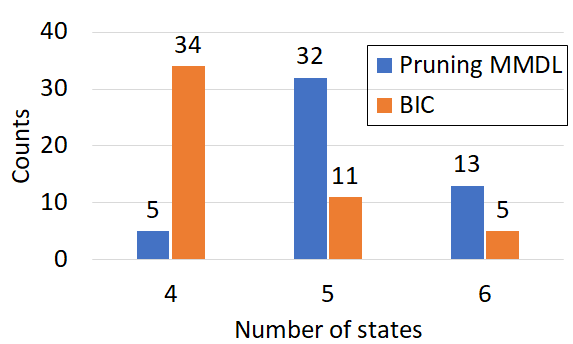
\includegraphics[height=25mm, trim={1.1in 0.1in 3in 0} ,scale=1]{hist_mmdl_bic1.png}
{
  \caption{Left: Histograms of the selected number of states for the standard BIC and pruning MMDL strategies for a total of 50 runs of the algorithm when the true underlying data is generated from 5 states; Right: Expected number of estimated states using a BIC and MMDL criterion respectively.}}
\end{minipage}
\begin{minipage}{0.45\columnwidth}
\hspace{-3mm}
\begin{tabular}{|l|c|c|}
%\footnotesize{
    \hline
    Method & Nº states & Nº iter. \\
    \hline\hline
    BIC &  $4.4\pm 0.7$  & $38.6\pm34.2$\\
    MMDL &  $5.2\pm 0.6$ & $5.8\pm 2.9$\\
    \hline
%    }
\end{tabular}
\end{minipage}
\end{figure}
\vspace*{-10pt}
\section{Conclusions and future work}
Experiments with synthetic data show that the pruning MMDL method for HSMMs provides a higher accuracy in the selection of the optimal number of states, when compared with BIC, and simultaneously a less demanding computational requirement. Future work concerns a more solid comparison with other methods such as the Akaike information criterion (AIC) and the method proposed in \citet{yu2015hidden}. Another important contribution would be to demonstrate the effectiveness in a more substantial application study, for example by using real data or by simulating synthetic data with some particularities that affect the learning process (e.g. observe the difference between parametric and non-parametric distributions, both in the state emissions and durations).

\footnotesize{
\bibliography{egbib}
}
\clearpage
\iffalse
\section{PROOF RECPAD 2019}
This appendix contains the proof of the equivalence between an HSMM \textbf{$\mu$} with $k$ states, where the duration probability of each state $S_i$ is a mixture of geometric distributions with parameters $\theta_{im}$ (see Section \ref{sec:hsmm})
and another HSMM \textbf{$\mu'$} with $k'$ states where the duration probability of each state is a single geometric distribution.
The HSMM model $\mu$ with emission and duration probabilities given by eqs. \eqref{poisson} and \eqref{mix_geom} is equivalent to another HSMM $\mu'$ with $k'=\sum_{i=1}^k M_i$ states where each state has only one geometric distribution %\textcolor{blue}{*"*}
to specify its duration. The equivalence is defined in terms of the likelihood of observations, i.e., $P(\textbf{O}|\mu)=P(\textbf{O}|\mu')$. \\ \noindent
In section \ref{d1} we will describe how model $\mu'$ is built and in section \ref{d2} we present the proof of the equivalence between both models.
\subsection{Building an equivalent HSMM model $\mu'$}
\label{d1}
Given the original HSMM model $\mu=(\mathbf{s},\boldsymbol{A},\boldsymbol{\pi},\boldsymbol{B},\boldsymbol{P})$, its equivalent model $\mu'=(\mathbf{s'},\boldsymbol{A'},\boldsymbol{\pi'},\boldsymbol{B'},\boldsymbol{P'})$ is built by splitting each state $s_i$ into $M_i$ states, one for each geometric distribution %\textcolor{blue}{*"*}
of the mixture. Thus we obtain $k'=\sum_{i=1}^k M_i$ states for model $\mu'$. The set of states of the new model is $S'=\{s'_1,...,s'_k\}=\{s'_{11},...,s'_{1M_1},s'_{21},...,s'_{2M_2},s'_{31},...,s'_{kM_k}\}$, where the double index notation in $s'_{kM_k}$ represents the ${M_k}^{th}$ geometric distribution %\textcolor{blue}{*"*}
of the original state $k$. The emission probability of each state $s'_{im}$
is the same as in eq. \eqref{poisson}. % due to the fact that the emission probability density function is conditionally independent on the component mixture given the corresponding state.
Regarding the state transition probability, using the double index notation, we have
\begin{equation}
    A'_{ikz,jmd} = A'_{ik,jmd} = A_{ij}c_{jm}p'_{jm}(d),
    \label{transition_mu'}
\end{equation}
representing the probability of going from state $s'_{ik}$ with duration $z$ to state $s'_{jm}$ with duration $d$. In eq. \eqref{transition_mu'}: the explicit duration HSMM assumption is exploited meaning that a state transition is independent to the duration of the previous state; $A_{ij}$ is the original state transition probability from $s_i$ to $s_j$; $c_{jm}$ is the mixing weight of the $m^{th}$ component from the original state $s_j$; and $p'_{jm}(d)$ is the probability of duration $d$ in state $s'_{jm}$, given by the geometric probability mass function in eq. \eqref{geom} with parameter $\theta_{jm}$.
%Notice that $A'_{ikz,jmd}$ does not depend on $k$ and 
%\textcolor{red}{(here is a bit of a confusion because duration d is discrete but the duration probability distribution here I assumed to be gaussian, therefore I used the integral over the duration, but maybe we need to use the discrete counterpart of gaussians)}
%\begin{equation}
%    \sum_{jmd} A'_{ikz,jmd} = \sum_{j=1}^k \sum_{m=1}^{M_j} \sum_{d=1}^D A_{ij} c_{jm}P'_{jm}(d).
%    \label{norm_trans_mu'_1}
%\end{equation}
%The duration probability $P'_{jm}(d)$ corresponds to the probability of observing duration $d$ while in state $S'_{jm}$ and is given the geometric probability mass function in \eqref{geom}.
%\begin{equation}
%    P'_{jm}(d)=P'(d|S'_{jm})=\mathcal{D}(d|\theta_{jm}).
%    \label{duration_mu'}
%\end{equation}
%Replacing eq. \eqref{duration_mu'} in \eqref{norm_trans_mu'_1}, yields the following result
%\begin{equation}
%    \sum_{jmd} A'_{ikz,jmd} =  \sum_{j=1}^k A_{ij} \sum_{m=1}^{M_j} c_{jm} \sum_{d=1}^D \mathcal{D}(d|\theta_{jm}) = 1,
%    \label{norm_trans_mu'_2}
%\end{equation}
%which proves that $A'_{ikz,jmd}$ normalizes to 1, as required.\\ \noindent
Finally, regarding the initial state probability, we define
\begin{equation}
    \pi'(s'_{jm}) = \pi(s_j)c_{jm},
    \label{pi_mu'}
\end{equation}
as the probability that state $s'_{jm}$ is the first state in the state sequence. %, which also normalizes to 1.
It can be easily confirmed that eqs. \eqref{transition_mu'} and \eqref{pi_mu'} normalize to 1, as required.
\subsection{Equivalence between HSMM models $\mu$ and $\mu'$}
\label{d2}
The proof of the equivalence between HSMM models $\mu$ and $\mu'$ uses the \textit{forward-backward} procedure to compute the likelihood of the observations, namely the forward variable of the explicit duration HSMM, defined and iteratively computed according to
\begin{equation}
\alpha_t(s_j) = P(\textbf{O}, S_{\rightarrow t|}=s_j;\mu) = \sum_{i=1}^k \sum_{d=1}^{d_{max}} \alpha_{t-d}(s_i)A_{ij}p_j(d)u_t(s_j,d),
    \label{forward_hsmm2}
\end{equation}
where $u_t(S_j,d)=\prod_{\tau=t-d+1}^t p(o_\tau|s_j)$ and the notation $S_{\rightarrow t|}=s_j$ means that state $s_j$ ends at time $t$. \\ \noindent
The likelihood of the observations for this model is given by
\begin{equation}
    P(\textbf{O}|\mu) = \sum_{j=1}^k \alpha_T(s_j).
     \label{likelihood_mu}
\end{equation}
Notice that the likelihood has the same expression as for ordinary HMMs \cite{rabiner1989tutorial}.
%Using this notation \textcolor{blue}{(later use the same notation in both sections!!!!)}, we have, for HSMM model $\mu$,
%\begin{equation}
%    \alpha_T(S_j) = \sum_{i=1}^k \sum_{d=1}^D \alpha_{T-d}(S_i)A_{ij}P_j(d)u_T(j,d),
%    \label{def_alpha_mu'}
%\end{equation}
Similarly, the likelihood of the observations for model $\mu'$ is
\begin{equation}
    P(\textbf{O}|\mu')=\sum_{j=1}^{k'} \alpha_T(s'_j)=\sum_{j=1}^k \sum_{m=1}^{M_j} \alpha_T(s'_{jm}),~
    \label{likelihood_mu'}
\end{equation}
that is, using the double index component notation introduced in Section \ref{d1}. In order to prove the equivalence between models $\mu$ and $\mu'$, in terms of the likelihoods of eqs. \eqref{likelihood_mu} and \eqref{likelihood_mu'}, we introduce the following variable
\begin{equation}
    \alpha'_T(s_j) = \sum_{m=1}^{M_j} \alpha_T(s'_{jm}).
    \label{def_components}
\end{equation}
The two models are equivalent if $\alpha'_T(s_j) = \alpha_T(s_j),  \forall j\in[k]$. 
The proof of is derived by induction on the length $T$ of the observation sequence.
\begin{proof}
For $T=1$, we have
\begin{equation}
    \alpha_1(s_j)= \underset{\textit{(d=1)}}{\sum_{i=1}^k\alpha_0(s_i)A_{ij}p_j(1)u_1(s_j,1)} = \sum_{i=1}^k \pi(s_i)A_{ij}p_j(1)p(o_1|s_j),
\end{equation}
for model $\mu$ and
\begin{equation}
    \alpha'_1(s_j) \underset{def}{=} \sum_{m=1}^{M_j} \alpha_1(s'_{jm}) = \underset{\textit{(d=1)}}{\sum_{m=1}^{M_j} \sum_{i=1}^k \sum_{l=1}^{M_l} \pi'(s'_{il}) A'_{il,jm1} p(o_1|s'_{jm})}
    \label{def_alpha1_mu'}
\end{equation}
for model $\mu'$. 
Replacing in eq. \eqref{def_alpha1_mu'} the definitions from eqs. \eqref{poisson}, \eqref{mix_geom}, \eqref{transition_mu'} and \eqref{pi_mu'} and
%\begin{equation}
%\alpha'_1(s_j) = \underset{(d=1)}{\sum_{m=1}^{M_j} \sum_{i=1}^k \sum_{l=1}^{M_l} \pi(s_i)c_{il} A_{ij}c_{jm} \mathcal{D}(1|\theta_{jm})b_j(O_1)}.
%\end{equation}
re-arranging terms by noticing that $\sum_{l=1}^{M_l} c_{il}=1$, yields
\begin{equation}
\alpha'_1(s_j) %= \underset{(d=1)}{b_j(O_1)\Bigg(\sum_{m=1}^{M_j}c_{jm}\mathcal{D}(1|\theta_{jm})\Bigg) \sum_{i=1}^k \pi(s_i) A_{ij}\Bigg(\sum_{l=1}^{M_l} c_{il}\Bigg)}
=\sum_{i=1}^k \pi(s_i)A_{ij}p_j(1)p(o_1|s_j).
\end{equation}
Therefore we can conclude that $\alpha'_1(s_j) \equiv \alpha_1(s_j), \forall j \in [k]$. \\ \noindent
To show the recursion, we need to prove the following implication
\begin{equation}
    \alpha_{T-d}(s_i)=\alpha'_{T-d}(s_i), \forall{d \in [d_{max}] \cap [1,T]} \implies \alpha_{T+1}(s_i) = \alpha'_{T+1}(s_i).
    \label{implication}
\end{equation}
From eq. \eqref{forward_hsmm2}, we know that
\begin{equation}
    \alpha_{T+1}(s_j) = \sum_{i=1}^k \sum_{d=1}^{d_{max}} \alpha_{T+1-d}(s_i)A_{ij}p_j(d)u_{T+1}(s_j,d).
    \label{alpha_T+1_mu}
\end{equation}
Likewise, for model $\mu'$, we have
\begin{equation}
    \alpha'_{T+1}(s_j)=\sum_{m=1}^{M_j} \alpha_{T+1}(s'_{jm}) = \sum_{m=1}^{M_j} \sum_{i=1}^k \sum_{l=1}^{M_l} \sum_{d=1}^{d_{max}} \alpha_{T+1-d}(s'_{il}) A'_{il,jmd}u_{T+1}(s'_{jm},d).
    \label{alpha_T+1_mu'_1}
\end{equation}
Invoking eqs. \eqref{mix_geom}, \eqref{transition_mu'}, \eqref{pi_mu'} and \eqref{def_components} and noticing that from eq.  \eqref{poisson} we can conclude that $u_{T+1}(s'_{jm},d)=u_{T+1}(s_j,d)$, eq. \eqref{alpha_T+1_mu'_1} simplifies to
%\begin{equation}
%   \alpha'_{T+1}(s_j)=\sum_{i=1}^k \sum_{d=1}^D u_{T+1}(j,d)A_{ij} \bigg(\sum_{m=1}^{M_j} c_{jm} \mathcal{D}(d|\theta_{jm})\Bigg) \bigg(\sum_{l=1}^{M_l} \alpha_{T+1-d}(S'_{il})\Bigg).
%    \label{alpha_T+1_mu'_2}
%\end{equation}
%Again, equation \eqref{alpha_T+1_mu'_2} can be further simplified by taking advantage of eqs. \eqref{duration_mu} and \eqref{def_components}, yielding
\begin{equation}
 \alpha'_{T+1}(s_j) = \sum_{i=1}^k \sum_{d=1}^{d_{max}} \alpha'_{T+1-d}(s_i)A_{ij}p_j(d)u_{T+1}(s_j,d).
  \label{alpha_T+1_mu'}
\end{equation}
Comparing \eqref{alpha_T+1_mu} and  \eqref{alpha_T+1_mu'}, it is clear that the implication in eq. \eqref{implication} is true. For example, evaluating \eqref{implication} for $T=1$ means that (for $d=1$, the only allowed duration) if $\alpha_{1}(s_i)=\alpha'_{1}(s_i)$ then $\alpha_{2}(s_i)=\alpha'_{2}(s_i)$. The former equality was deducted in the first part of our proof, which implies the latter. Subsequently, evaluating \eqref{implication} for $T=2$ means that (for $d=[1,2]$) if $\alpha_{1}(s_i)=\alpha'_{1}(s_i)$ and $\alpha_{2}(s_i)=\alpha'_{2}(s_i)$ then $\alpha_{3}(s_i)=\alpha'_{3}(s_i)$. Both premises are guaranteed from the first proof and from the conclusions of the previous implication. Thus, the conclusion is met and the recursion continues until the condition is met for all $T$. \\ \noindent
This concludes our proof that $\alpha'_T(s_j)=\alpha_T(s_j)$ and, consequently, the models are likelihood-equivalent.
\end{proof}
\fi
\end{document}
